% Relatório referente ao projeto "Reconhecimento de Locutor Independente de
% Texto" entregue em 4 de Agosto de 2014, da disciplina "Processamento de Voz",
% ministrada pelo professor Tsang Ing Ren. O documento está no formato de paper
% do IEEE.

\documentclass[a4paper,twocolumn]{article}

\usepackage{times}
\usepackage[utf8]{inputenc}
\usepackage[english]{babel}
\usepackage[a4paper,margin=2cm,columnsep=1cm]{geometry}
\usepackage{authblk}
\usepackage{titlesec}
\usepackage[pdftex]{graphicx}
\usepackage{mathtools}


\begin{document}

\graphicspath{{images/}}
\renewcommand{\abstractname}{\normalsize\bfseries\filcenter ABSTRACT}
\titleformat*{\section}{\normalsize\bfseries\filcenter}
\titleformat*{\subsection}{\normalsize\bfseries\filcenter}
\renewcommand{\refname}{\normalsize\bfseries\filcenter REFERENCES}
\renewcommand{\figurename}{\small Figure}
\newcommand{\figureref}[1]{Fig. (\ref{fig:#1})}
\newcommand{\equationref}[1]{Eq. (\ref{eq:#1})}
\newcommand{\bigsum}{\displaystyle\sum}


\title{\textbf{Speaker Verification Using Adapted Gaussian Mixture Models}}
\author{\textit{Sérgio R. F. Vieira, Eduardo M. B. de A. Tenório and Tsang Ing Ren}}
\affil{Centro de Informática, Universidade Federal de Pernambuco\\
Recife, PE, Brazil -- www.cin.ufpe.br\\
\small\texttt{\{srfv,embat,tir\}@cin.ufpe.br}}
\date{August, 2014}

\maketitle


\begin{abstract}
\begin{itshape}
Colocar o abstract aqui

\noindent\textbf{keywords}: colocar keywords aqui
\end{itshape}
\end{abstract}


\section{INTRODUCTION}
\label{intro}

Traditionally, strategies for verification and identification of a individual are based on some foreknowledge, like a password or a personal identification number. In other cases physical objects are used (keys, cards, etc.). The Achilles heel of these strategies is the verification/identification object itself. Once a key is lost or a password is forgotten, the person cannot prove to be herself. In cases of theft, a malicious agent can easily impersonate the victim.

With the growing advancements in IT, biometric systems became more common and, in a self fed loop, more precise. The biometry of the voice is one of the most reliable and easy to use. To extract its features the person just needs to speak, and if the system is well designed it is very unlikely to an imposter be granted access. Many techniques based on statistical models exists, each one focused in a particular set of subproblems. Here we will use the Gaussian Mixture Models (GMM).

A GMM is a generic probabilistic model for multivariate densities capable of representing arbitrary densities, making it well suited for unconstrained text-independent applications. The use of GMMs for this type of speaker identification was first described in \cite{rose_reynolds_1990}, and since then this approach has gained popularity and became the state of the art in text-independent speaker recognition applications. This fact is evidenced by numerous papers published in majors conferences, such as International Conference on Acoustics, Speech, and Signal Processing (ICASSP), the International Speech Communication Association (ISCA, formerly known as Eurospeech), and the International Conference on Spoken Language Processing (ICSLP), as well as articles in ESCA Transactions on Speech Communications and IEEE Transactions on Speech and Audio Processing.

This paper is a reduced reproduction of \cite{reynolds_et_al_2000}, in which we present a Gaussian Mixture Model-Universal Background Model (GMM-UBM) and a GMM adapted from the GMM-UBM. These models are used to verify a speaker using the Likelihood-Ratio Test. The rest of the paper is devided in an explanation of the Likelihood Test, the GMM-UBM Verification System, the Experiments and later, the Conclusion.


\section{LIKELIHOOD TEST}
\label{likelihood_test}

Given a speech $Y$ and a speaker $S$, the speaker detection test can be restated as a basic hypothesis test between $H_0$ and $H_1$, where

\begin{description}\itemsep 0pt \parskip 1pt
    \item[$H_0$:] $Y$ is from the hypothesized speaker $S$
    \item[$H_1$:] $Y$ is \underline{not} from the hypothesized speaker $S$
\end{description}

\noindent The optimal test to decide between these two hypotheses is a likelihood ratio test given by

\begin{equation}
    \label{eq:likelihood_ratio_test}
    \frac{p(Y|H_0)}{p(Y|H_1)} = \left\{
        \begin{array}{l l}
        \geq \theta \quad\quad\quad \text{accept $H_0$}\\
        < \theta \quad\quad\quad \text{reject $H_0$}
        \end{array} \right.
\end{equation}

\noindent Naming the model for $H_0$ as $\lambda_{hyp}$, and the model for $H_1$ as $\lambda_{\overline{hyp}}$, the logarithm of \equationref{likelihood_ratio_test} is given by

\begin{equation}
    \label{eq:log_likelihood_ratio_test}
    \Lambda(X) = \log p(X|\lambda_{hyp}) - \log p(X|\lambda_{\overline{hyp}})
\end{equation}

The figure below is a simple diagram showing how the speaker detection system is organized. First the speech signal is preprocessed, with a vector of features extracted. These features are used to create the models for the speaker ($\lambda_{hyp}$) and the background ($\lambda_{\overline{hyp}}$). Later, the likelihood from each model is calculated and compared to classify the speech segment $Y$ as spoken or not by the speaker $S$.

\begin{figure}[h]
    \label{fig:speaker_detection_system}
    \centering
    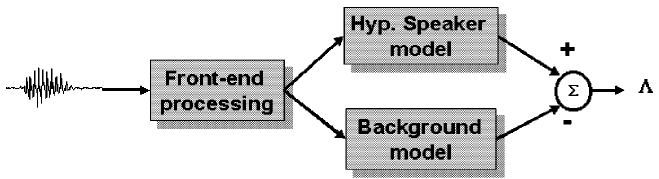
\includegraphics[scale=0.3]{speaker-detection-system}
    \caption{\textit{Likelihood ratio-based speaker detection system.}}
\end{figure}


\section{GMM-UBM VERIFICATION SYSTEM}

\subsection{Gaussian Mixture Models}

A GMM is a weighted sum of M mixture components of multivariate Gaussians. For a $D$-dimensional feature vector $\vec{x}$, the mixture density used for the likelihood function is defined as

\begin{equation}
    \label{eq:gmm_likelihood}
    p(\vec{x}|\lambda) = \sum_{i=1}^M w_i p_i(\vec{x})
\end{equation}

\noindent a weighted linear combination of $M$ unimodal Gaussian densities, $p_i(\vec{x})$, each parameterized by a mean $D\times 1$ vector, $\mu_i$ , and a $D\times D$ covariance matrix, $\Sigma_i$;

\begin{equation}
    \label{eq:gmm}
    p_i(\vec{x}) = \frac{1}{(2\pi)^\frac{D}{2}|\Sigma_i|^\frac{1}{2}}e^{-\frac{1}{2}(\vec{x} - \vec{\mu_i})'(\Sigma_i)^{-1}(\vec{x} - \vec{\mu_i})}
\end{equation}

\noindent and satisfying the constraint $\sum_{i=1}^M w_i = 1$. Experimental results showed that the best $\Sigma_i$ is a diagonal matrix, because it produces a better computation performance. Given the training vectors, the maximum likelihood model parameters are estimated using the iterative expectation-maximization (EM) algorithm, refining the GMM parameters to monotonically increase the likelihood of the estimated model for the observed feature vectors.

Given a utterance $X$ divided in independent vectors $X = \{\vec{x_1}, \dots, \vec{x_T}\}$, where each $\vec{x_t}$ is a vector of MFCCs for a frame $t$, the average loglikelihood of a model $\lambda$ is computed as

\begin{equation}
    \label{eq:loglikelihood_lambda}
    \log p(X|\lambda)_{avg} = \frac{1}{T}\sum_{t=1}^T \log p(\vec{x_t}|\lambda)
\end{equation}

\noindent where $\log p(\vec{x_t}|\lambda)$ is computed as in \equationref{gmm_likelihood}. For a corpus with more than one utterance, $X$ is the concatenation of the various utterances.

\subsection{Front-End Processing}

The front-end analysis occurs in several steps. First, the speech is segmented into frames by a 20-ms window progressing at a 10-ms frame rate. A speech activity detector is then used to discard silence–noise frames. Later the features are extracted.

The features extraction process transforms a speech signal into a vector containing the information needed to perform the verification/identification. In the case of text-independent verification, as shown in \cite{pinheiro_2013}, the features extracted must have: high variation inter-speakers and low variation intra-speakers; robustness in the presence of noise and distortion; be frequent and natural in speech; easy to measure and to extract from speech signal; hard to be artificially produced; be immutable, even in the presence of sickness or aging.

In this paper we used the Mel-Frequency Cepstral Coefficients (MFCCs) \cite{davis_mermelstein_1980} to perform the feature extraction, associated to their time derivatives and to the logarithm of the signal's energy. The Mel scale is derived from researches in human listening and is given by

\begin{equation}
    \label{eq:hertz_to_mel}
    mel = 2595\log_{10} (1 + \frac{f}{700})
\end{equation}

\noindent where \textit{f} is the frequency in Hertz. The log-scale improves the readability of lower frequencies, making it well suited for this kind of problem (the majority of human voice is under 4kHz). Details about the MFCCs extraction can be found in \cite{pinheiro_2013}.

\subsection{Universal Background Model}

In the GMM-UBM system we use a single, speaker-independent background model to represent $p(X|\lambda_{\overline{hyp}})$. The UBM is a large GMM trained to represent the speaker-independent distribution of features.

The approach of UBM training depends of the kind of data needed to classify. If the gender of the speaker to be identified is known a priori, there is no sense in test it against a UBM for the other gender (unless when testing the system's robustness). There are two approachs, as shown in the figure below.

\begin{figure}[h]
    \label{fig:gmm_ubm_training}
    \centering
    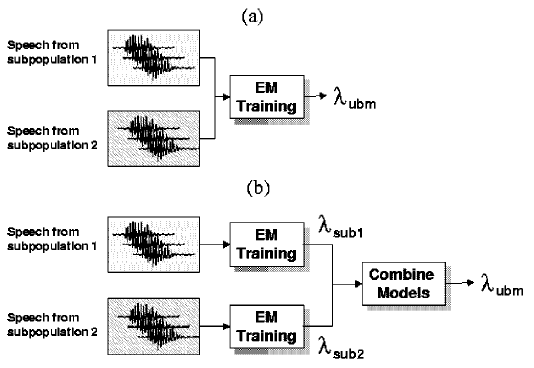
\includegraphics[scale=0.4]{gmm-ubm-training}
    \caption{\textit{Training of UBM with separation (b) and no separation (a) of gender.}}
\end{figure}

\noindent Notice the training is performed using the EM algorithm, as shown in \cite{dempster_1977}. Commonly the training algorithm for a model $\lambda$ stops when $p(X|\lambda^{(k)}) - p(X|\lambda^k) < 10^{-5}$.

\subsection{Adaptation of Speaker Model}

The logical approach is to train a pair of speaker model and UBM for each speaker. This way, we can guarantee that the speaker model is the best representation of the speaker and the UBM (without the speaker utterances) is the best representation for the rest. However, this approach is too expensive and doesn't show any significant advantage.

The best way to create a speaker model is by adaptation from a well-trained UBM. This provides a tighter coupling between the speaker’s model and UBM which not only produces better performance than decoupled models, but, as discussed later in this section, also allows for a fast-scoring technique. Like the EM algorithm, the adaption is a two step estimation process. The first step is identical to the expectation step of the EM algorithm, where estimates of the sufficient statistics of the speaker’s training data are computed for each mixture in the UBM. Unlike the second step of the EM algorithm, for adaptation these new sufficient statistic estimates are then combined with the old sufficient statistics from the UBM mixture parameters using a data-dependent mixing coefficient.

Given a UBM and training vectors from the hypothesized speaker, X = {x1 , . . . , xT }, we first determine the probabilistic alignment of the training vectors into the UBM mixture components

\begin{equation}
    \label{eq:prob_alignment}
    Pr(i|\vec{x_t}) = \frac{w_i p_i(\vec{x_t})}{\sum_{j=1}^M w_j p_j(\vec{x_t})}
\end{equation}

\noindent We then use \equationref{prob_alignment} to compute the sufficient statistics for the weight, mean, and variance parameters:

\begin{equation}
    \label{eq:sum_prob_alignment}
    n_i = \sum_{t=1}^TPr(i|\vec{x_t})
\end{equation}

\begin{equation}
    \label{eq:mean_new}
    E_i(\vec{x}) = \frac{1}{n_i} \sum_{t=1}^T Pr(i|\vec{x_t})\vec{x_t}
\end{equation}

\begin{equation}
    \label{eq:var_new}
    E_i(\vec{x}^2) = \frac{1}{n_i} \sum_{t=1}^T Pr(i|\vec{x_t})\vec{x_t}^2
\end{equation}

Finally, these new sufficient statistics from the training data are used to update the old UBM sufficient statistics for mixture i to create the adapted parameters for mixture $i$ with the equations:

\begin{equation}
    \label{eq:weight_adapt}
    \hat{w_i} = [\alpha_i \frac{n_i}{T} + (1 - \alpha_i)w_i]\gamma
\end{equation}

\begin{equation}
    \label{eq:mean_adapt}
    \vec{\hat{\mu_i}} = \alpha_i E_i(\vec{x}) + (1 - \alpha_i)\vec{\mu_i}
\end{equation}

\begin{equation}
    \label{eq:var_adapt}
    \vec{\hat{\sigma_i^2}} = \alpha_i E_i(\vec{x^2}) + (1 - \alpha_i)(\vec{\sigma_i^2} + \vec{\mu_i^2}) - \vec{\hat{\mu_i^2}}
\end{equation}

The coefficient $\alpha_i$ controls the balance between old and new estimates. The scale factor, $\gamma$, is computed over all adapted mixture weights to ensure they sum to unity. The $\alpha_i$ coefficient is defined as

\begin{equation}
    \label{eq:alpha_coeff}
    \alpha_i = \frac{n_i}{n_i + r}
\end{equation}

\noindent where $r$ is a fixed relevance factor. The coefficient $\alpha_i$ is between 0 and 1. When close to 0, the adaptation is minimum, and when close to 1, the new parameters are more emphasised. A common value for the relevance factor is $r = 16$.

Since the adaptation is data dependent, not all Gaussians in the UBM are adapted during speaker model training. Knowing the amount of unadapted Gaussians can be an important factor in reduced model storage requirements, since it is possible to efficiently store models using only the difference with the UBM.

\subsection{Log-Likelihood Ratio Computation}

The log-likelihood ratio for a test sequence of feature vectors $X$ is computed as $\Lambda(X) = \log p(X|\lambda_{hyp}) - \log p(X|\lambda_{\overline{hyp}})$. The fact that the hypothesized speaker model was adapted from the UBM, however, allows a faster scoring method than merely evaluating the two GMMs. This fast scoring approach is based on two observed effects. The first is that when a large GMM is evaluated for a feature vector, only a few of the mixtures contribute significantly to the likelihood value. This is because the GMM represents a distribution over a large space but a single vector will be near only a few components of the GMM. Thus, likelihood values can be approximated very well using only the top $C$ best scoring mixture components.

The second observed effect is that the components of the adapted GMM retain a correspondence with the mixtures of the UBM, so that vectors close to a particular mixture in the UBM will also be close to the corresponding mixture in the speaker model. Using these two effects, a fast scoring procedure operates as follows: For each feature vector, determine the top $C$ scoring mixtures in the UBM and compute UBM likelihood using only these top $C$ mixtures. Next, score the vector against only the corresponding $C$ components in the adapted speaker model to evaluate the speaker’s likelihood. For a UBM with $M$ mixtures, this requires only $M + C$ Gaussian computations per feature vector compared to $2M$ Gaussian computations for normal likelihood ratio evaluation. When there are multiple hypothesized speaker models for each test segment, the savings become even greater. In the GMM-UBM system, we use a value of $C = 5$.


\section{EXPERIMENTS}


\section{CONCLUSION}


\begin{thebibliography}{9}
    \bibitem{rose_reynolds_1990}
        R. C. Rose and D. A. Reynolds,
        ``Text-independent speaker identification using automatic acoustic segmentation,"
        in \textit{Proc. of the International Conference on Acoustics, Speech, and
        Signal Processing},
        1990,
        pp. 293–296.

    \bibitem{reynolds_et_al_2000}
        D. A. Reynolds et al.,
        ``Speaker verification using adapted gaussian mixture models,"
        \textit{Digital Signal Processing}, vol. 10,
        (1-3) pp. 19-41,
        2000.

    \bibitem{pinheiro_2013}
        H. N. B. Pinheiro,
        ``Sistemas de reconhecimento de locutor independente de texto,"
        B.Eng. monograph, Universidade Federal de Pernambuco,
        Recife, Pernambuco, Brazil,
        2013.

    \bibitem{davis_mermelstein_1980}
        S. B. Davis and P. Mermelstein,
        ``Comparison of Parametric Representations for Monosyllabic Word Recognition in Continuously Spoken Sentences,"
        in \textit{IEEE Trans. Acoust., Speech, Signal Process.},
        vol. 28
        pp. 357-366,
        Aug. 1980.

    \bibitem{dempster_1977}
        A. Dempster et al.,
        Maximum likelihood from incomplete data via the EM algorithm,
        \textit{J. Roy. Stat. Soc.} \textbf{39} (1977), 1–38.

    \bibitem{corpus_paper}
        R. H. Woo et al.,
        ``The MIT Mobile Device Speaker Verification Corpus: Data Collection and Preliminary Experiments,"
        in \textit{The Speaker and Language Recognition Workshop (IEEE Odyssey 2006),}
        San Juan, Puerto Rico, 2006.

\end{thebibliography}

\end{document}